\documentclass{standalone}
\usepackage{tikz}

\definecolor{viridisblue}{RGB}{68,1,84}
\definecolor{viridisyellow}{RGB}{253,231,37}
\definecolor{viridisgreen}{RGB}{35,138,141}

\begin{document}

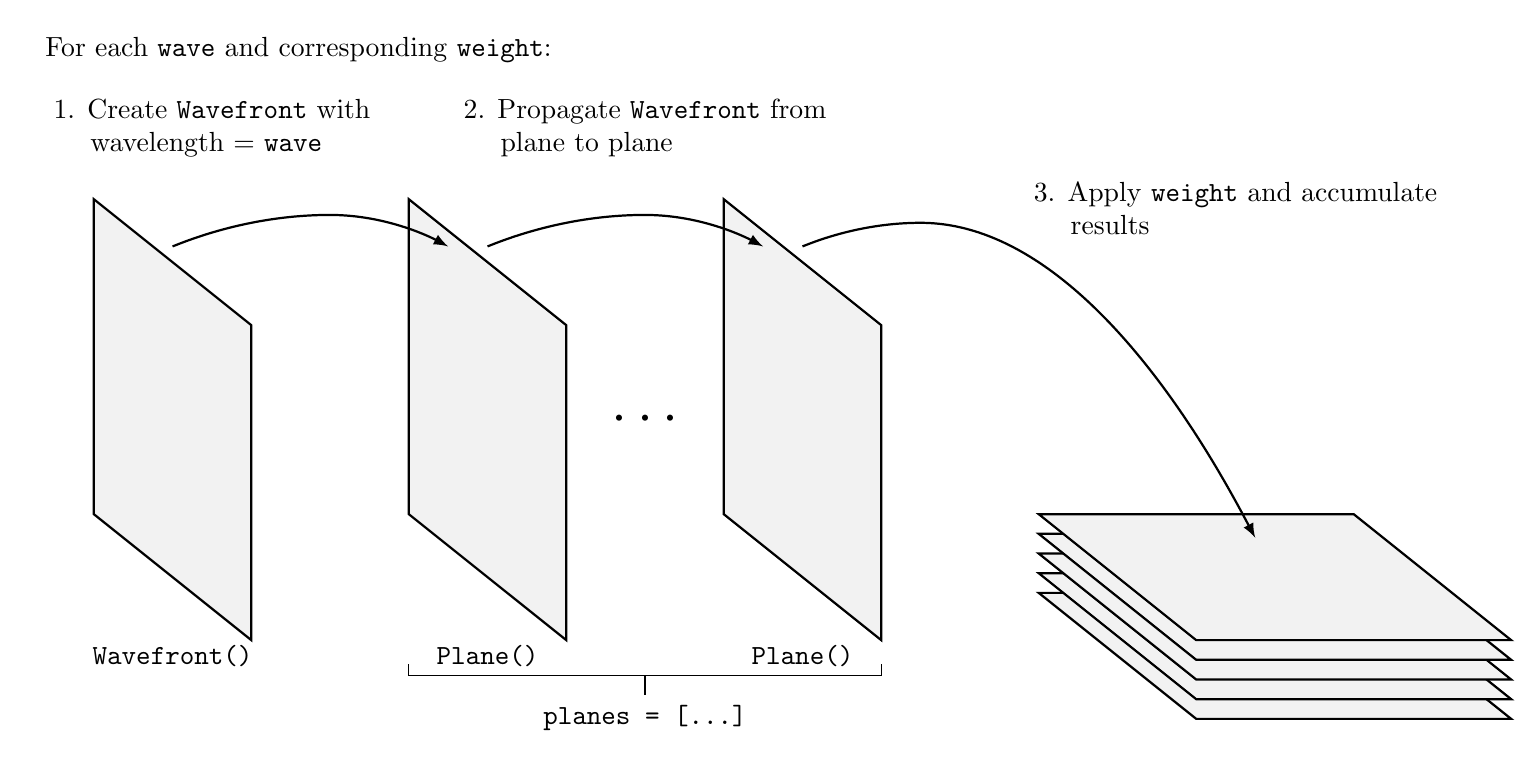
\begin{tikzpicture}[z={(1cm,0cm)},x={(0.5cm,-0.4cm)}, y={(0cm,1cm)}, scale=1]

    % constants
    \def\zwf{0}
    \def\zpa{4}
    \def\zpb{8}
    \def\zpc{12}
    \def\zpcc{16}

    % wavefront
    \draw [thick,fill=black!5] (-2,-2,\zwf) -- (2,-2,\zwf) -- (2,2,\zwf) -- (-2,2,\zwf) -- cycle; 
    \node [align=center] at (-1,3.3,1) {\begin{tabular}{l}1. Create \texttt{Wavefront} with \\ \hspace{1em} wavelength = \texttt{wave}\end{tabular}};
    \node [align=center] at (0,-3,\zwf) {\texttt{Wavefront()}};


    \draw [thick,fill=black!5] (-2,-2,\zpa) -- (2,-2,\zpa) -- (2,2,\zpa) -- (-2,2,\zpa) -- cycle; 
    \node [align=center] at (0-1,3.3,6.5) {\begin{tabular}{l}2. Propagate \texttt{Wavefront} from\\ \hspace{1em} plane to plane\end{tabular}};
    \node [align=center] at (0,-3,\zpa) {\texttt{Plane()}};

    \draw [-latex, thick] (0,2.2,\zwf) parabola bend (0,2.6,2) (0,2.2,3.5);
    \node [align=center] at (0,0,6) {\huge $\cdots$};
    
    \draw [thick,fill=black!5] (-2,-2,\zpb) -- (2,-2,\zpb) -- (2,2,\zpb) -- (-2,2,\zpb) -- cycle; 
    \node [align=center] at (0,-3,\zpb) {\texttt{Plane()}};

    \draw (0,-3.25,3) -- (0,-3.25,9);
    \draw (0,-3.25,3) -- (0,-3.1,3);
    \draw (0,-3.25,9) -- (0,-3.1,9);
    \draw (0,-3.25,6) -- (0,-3.5,6);
    \node [align=center, below] at (0,-3.5,6) {\texttt{planes = [...]}};
    
    \draw [-latex, thick] (0,2.2,\zpa) parabola bend (0,2.6,6) (0,2.2,7.5);
    \draw [thick,fill=black!5] (-2,-3,\zpc) -- (-2,-3,\zpcc) -- (2,-3,\zpcc) -- (2,-3,\zpc) -- cycle; 
    \draw [thick,fill=black!5] (-2,-2.75,\zpc) -- (-2,-2.75,\zpcc) -- (2,-2.75,\zpcc) -- (2,-2.75,\zpc) -- cycle; 
    \draw [thick,fill=black!5] (-2,-2.5,\zpc) -- (-2,-2.5,\zpcc) -- (2,-2.5,\zpcc) -- (2,-2.5,\zpc) -- cycle; 
    \draw [thick,fill=black!5] (-2,-2.25,\zpc) -- (-2,-2.25,\zpcc) -- (2,-2.25,\zpcc) -- (2,-2.25,\zpc) -- cycle; 
    \draw [thick,fill=black!5] (-2,-2,\zpc) -- (-2,-2,\zpcc) -- (2,-2,\zpcc) -- (2,-2,\zpc) -- cycle; 
    
    \draw [-latex, thick] (0,2.2,\zpb) parabola bend (0,2.5,9.5) (0,-1.5,13.75);

    \node [align=left] at (-1,4.3,2.1) {For each \texttt{wave} and corresponding \texttt{weight}:};
    %\draw [thick,dashed] (0,5.25,-2) -- (0,5.25,10) -- (0,-4.1,10) -- (0,-4.1,-2) -- cycle; 


    \node [align=center] at (-1,2.25,14) {\begin{tabular}{l}3. Apply \texttt{weight} and accumulate \\ \hspace{1em} results\end{tabular}};



\end{tikzpicture}

\end{document}
